\documentclass[ignoreonframetext,unicode]{beamer}

\usepackage[utf8]{inputenc}
\usepackage[T1]{fontenc}
\usepackage[english,russian]{babel}
\usepackage{graphicx,pgf}
\usepackage{multimedia}
\usepackage{amsmath}
\usepackage{amssymb}
\usepackage{amsfonts}
\usepackage{mathtools}

%\usepackage[oglav,spisok,boldsect,eqwhole,figwhole,hyperref,hyperprint,remarks,greekit]{fn2kursstyle}

\graphicspath{
	{./style/}
	{../wolfram/f_22600_10.08.26/plots/}
	{../wolfram/f_22601_10.08.26/plots/}
	{../wolfram/f_22609_10.08.25/plots/}
	{../wolfram/f_22608_10.08.28/plots/}
	{./illustr/}
}

\usetheme{Warsaw}

\useinnertheme{circles}   %внутренняя тема
%\useoutertheme{smoothbars}   %внешняя тема
\usecolortheme{seahorse}     %цветовая схема
%\usefonttheme{serif}    %шрифты
%\defbeamertemplate*{footline}{shadow theme}
%\setbeameroption{hide notes}
\usepackage[document]{ragged2e}

%%Полужирный наклонный шрифт в формулах
\newcommand\be[1]{\text{\mathversion{bold}${#1}$}}
\newcommand\bi[1]{\text{\mathversion{bold}${#1}$}}
\newcommand\mathbi[1]{\text{\mathversion{bold}${#1}$}}

%номера слайдов
\newcommand*\oldmacro{}%
\let\oldmacro\insertshorttitle%
\renewcommand*\insertshorttitle{%
	\oldmacro\hfill%
	\insertframenumber\,/\,\inserttotalframenumber}
\RequirePackage{caption}
\DeclareCaptionLabelSeparator{defffis}{ }
\captionsetup{justification=centering,labelsep=defffis}

%\title{Курсовая работа}
%\subtitle{Численные схемы для аппроксимации неограниченных решений при моделировании обтекания профиля крыла в вихревых методах}
\title{Линейная аппроксимация зашумленных данных}
\author[Егоров А.\,Д.]{Докладчик: Егоров А.\,Д.\and\\[0.5mm] Научный руководитель: Казаков К.\,Е.}

\institute[каф. Прикладная математика ФН-2]{группа ФН2-52Б}
\date{\today}
\titlegraphic{
\includegraphics[width=2cm]{emblema.pdf}}
%\renewcommand{\vec}[1]{\text{\mathversion{bold}${#1}$}}

\begin{document}
	
	\begin{frame}[plain]
		\maketitle
		%\insertshortinstitute{Группа ФН2-41Б}
	\end{frame}

%\begin{frame}{Введение}
	
%	Данные, полученные во время реального эксперимента, часто являются весьма не точными, так как при считывании показаний с датчиков, сигнал всегда приходит с шумами. Причиной возникновения шума может стать что угодно: будь то перебой связи или сильная тряска. Следовательно, возникает необходимость в его подавлении и аппроксимации полученных данных.
	
%	Задача, рассматриваемая в этой работе, пришла из транспортной отрасли, из сферы перевозки грузов, где необходимо отслеживать уровень топлива задействованного автомобиля.
	
%\end{frame}

\begin{frame}{Постановка задачи}
	\small
	%\begin{columns}\vspace*{-2.0mm}
	%	\column{0.5\textwidth}			
	\begin{block}{Задача}
		Требуется обработать экспериментально полученный график функции при условии, что в процессе измерений наблюдаются шумы. Необходимо построить линейную аппроксимацию графика, которая убирает шумы и позволяет достаточно точно определить как места существенного возрастания или убывания функции, так и величины этих изменений. Рассмотреть случай, когда функция не обладает периодичностью.
	\end{block}
			
	\center
	\includegraphics[width=0.65\textwidth]{f_22608_10.08.28_data.pdf}
		
	\normalsize
\end{frame}

%\begin{frame}{Фильтрация исходных данных}
%		Необходимо отбросить следующие точки:
%		\begin{itemize}
	%		\item ошибки датчика (точки, значения в которых сильно отличаются от среднего значения на всем отрезке),
	%		\item залипания датчика (отрезки, на которых показания датчика неизменны, т.е. отличаются не более чем на $1 \%$).
%		\end{itemize}
%		\center
%		\includegraphics[width=1.\textwidth]{f_22608_10.08.28_data_raw_filtered_comparison.pdf}
	
%\end{frame}



\begin{frame}{Построение непрерывной кусочно-линейной аппроксимирующей функции}
	\small
	
	Для отрезка $[a, b] \in \mathbb{R}$ существует
	некоторая неизвестная функция $F\!: [a, b]  \rightarrow \mathbb{R}$ и 
	%$X = \{x_0, x_1, \dots, x_n\}$,  %Датчик проводит замеры раз в 15 секунд, т.е. 
	задан набор точек  $\eta = \left\{(x_i, y_i) \right\}_{i=0}^{n}$, такой что
	\vspace*{-2.mm}
	\begin{gather*}
		%Z =\left\{(x_0, y_0), (x_1, y_1),\dots, (x_n, y_n)  \right\}, \\
		a = x_0 < x_1 < \cdots < x_n = b, \quad y_i  = F(x_i), \quad i = 0, \dots, n.
	\end{gather*}
	
	%Исходные данные аппроксимируются кусочно-линейной функцией с меньшим числом узлов, за счет чего уменьшается количество шума. 
%\vspace*{-2.mm}
%$= \{\xi_0, \xi_1, \dots, \xi_m \} ,  \ $
	\vspace*{-2.mm}
	Для $\eta$ выбирается сетка 
	$\xi = \{\xi_k\}_{k=0}^{m}, \ (m < n).$
	\center
	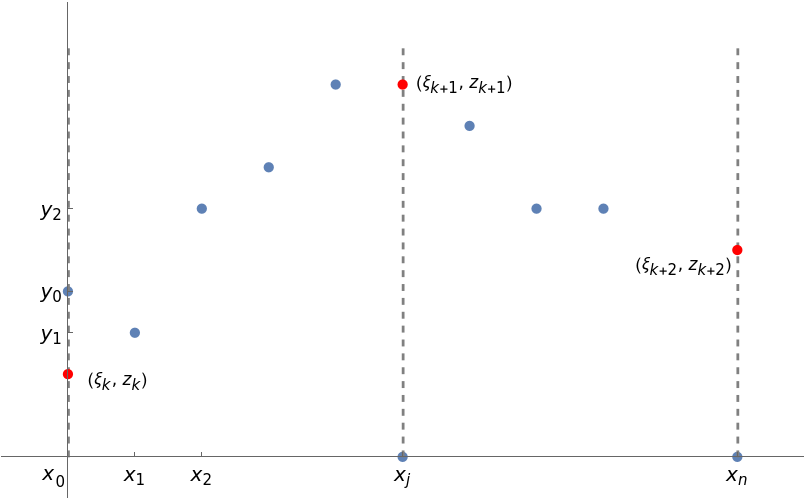
\includegraphics[width=0.6\textwidth]{illustr_spline.png}
	\vspace*{-2.mm}
	\flushleft
	Необходимо найти вертикальные координаты $z_k$ в соответствующих точек $\xi_k$.
	\normalsize
\end{frame}

%\begin{frame}{Построение непрерывной кусочно-линейной аппроксимирующей функции}
%	\small
%	Исходные данные аппроксимируются кусочно-линейной функцией с меньшим числом узлов, за счет чего уменьшается количество шума. 
%	\vspace*{-2.mm}
	
%	Для набора точек 
%	$\{(x_i, y_i)\}_{i=0}^{n} =\{ (x_0, y_0), (x_1, y_1) \dots (x_n, y_n)\},$
	
%	\vspace*{2.mm}
%	выбирается сетка
%	$\{\xi_k\}_{k=0}^{m} = \{\xi_0, \xi_1, \dots, \xi_m \} ,  \ (m < n).$
%	\center
%	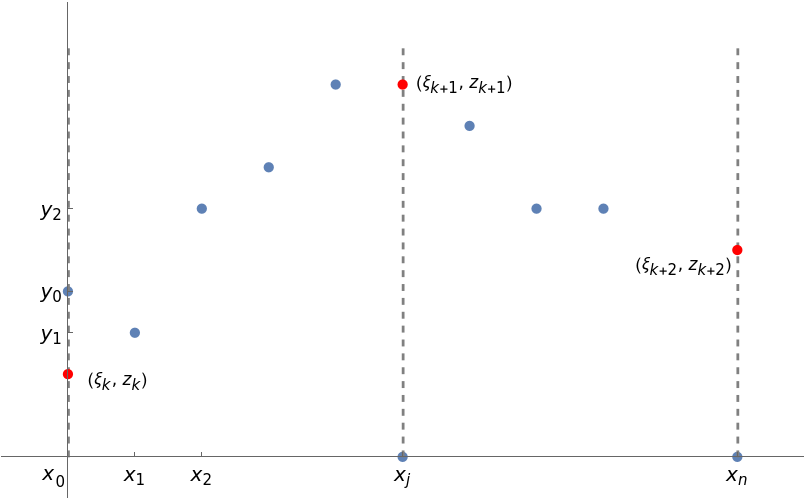
\includegraphics[width=0.5\textwidth]{illustr_spline.png}
	%
%	\flushleft
%	Необходимо найти вертикальные координаты $z_k$ в соответствующих точек $\xi_k$.
%	\normalsize
%\end{frame}



\begin{frame}{}%{Построение непрерывной кусочно-линейной аппроксимирующей функции}
	\small
	
	%Координату $z_k$ будем искать из следующих соображений:
	%есть набор из $r$ точек $ \{(x_{k, j}, y_{k, j})\}_{j=0}^{r} $ принадлежащих участку  $ ( \xi_k, \xi_{k+1} ) $, всего таких наборов $m$ штук.	
	Для нахождения $z_k$ будем минимизировать квадраты отклонений точек, принадлежащих участку  $ [ \xi_k, \xi_{k+1} ] $, от прямой $p$, соединяющей
	точки $ (\xi_k, z_k)$ и $(\xi_{k+1} , z_{k+1})$:
	\vspace*{-2.mm}
	
	\begin{equation}
			(z_{k,0} - y_{k, 0})^2 + (z_{k,1} - y_{k, 1})^2 + (z_{k,2} - y_{k, 2})^2 + \dots + (z_{k, r_k} - y_{k, r_k})^2 \rightarrow min, 
	\label{min_eq}
	\end{equation}
	\,\ $k=\overline{0,m},$
	
	\vspace*{1.mm}
	где $r_k$ --- количество точек из $\eta$ принадлежащих участку  $ [ \xi_k, \xi_{k+1} ]$, \\
	$z_{k,j}$ --- координата соответствующая значению прямой $p$ в точке $x_{k, j}$, ее находим из следующих уравнений:
	\begin{equation*}
		z_{k,0} = z_k, \ \ 
		z_{k,j} = \dfrac{z_{k+1}-z_{k}}{\xi_{k+1} - \xi_k} x_{k, j} -  \dfrac{z_{k+1}-z_{k}}{\xi_{k+1} - \xi_k} \xi_{k} + z_k, \ \ 
		z_{k,r_k} = z_{k+1}.
	\end{equation*}

	
	\normalsize
\end{frame}



\begin{frame}{}%{Линейный сплайн}
	\small
	Из (\refeq{min_eq}) получим систему линейных алгебраических уравнений относительно $\{z_k\}_{k=0}^m$:
	\begin{equation*}
		%\label{spline_sys}
		\begin{dcases}
			\dfrac{\partial}{\partial{z_0}} \Big[(z_{0,0} - y_{0,0})^2 + (z_{0,1} - y_{0,1})^2  + \dots + (z_{0,r_0} - y_{0,r_0})^2 \Big] = 0,\\				
			\dfrac{\partial}{\partial{z_1}}\Big[	(z_{1,0} - y_{1,0})^2 + (z_{1,1} - y_{1,1})^2  + \dots + (z_{1,r_1} - y_{1,r_1})^2 \Big]= 0,\\
			\dotsm \\
			\dfrac{\partial}{\partial{z_{m\!-\!1}}} \Big[	(z_{m\!-\!1,0} - y_{m\!-\!1,0})^2 + \dots + (z_{m\!-\!1,r_{m-1}} - y_{m\!-\!1,r_{m-1}})^2 \Big]= 0,\\				
			\dfrac{\partial}{\partial{z_{m}}} \Big[ 	(z_{m,0} - y_{m,0})^2 \Big]= 0,\\				
		\end{dcases}			
	\end{equation*}
	решением которой будут требуемые нам координаты. Cтоит отметить, что матрица
	данной системы двухдиагональна.
	\normalsize
	
\end{frame}

\begin{frame}{Начальная сетка}
	Сетку будем строить с определенным шагом $\mathrm{d\xi}$ так, чтобы\ \ \ \  узлы сетки совпадали с некоторым точками и чтобы на участке была хотя бы 1 точка.
	%, но дополнительно будем учитывать, что данные распределены неравномерно: мы будем увеличивать интервал до тех пор, пока он не станет больше $\mathrm{d\xi}$ и на нем не будет как минимум 1 точка.
	
	\center
	\includegraphics[width=0.9\textwidth]{f_22608_10.08.28_uni.pdf}
	
	
\end{frame}

\begin{frame}{Модифицированная сетка}
	\begin{block}{Модификации}
		\begin{itemize}
			\item размещение узлов в точках максимума и минимума начальных данных,
			\item размещение узлов в точках максимума и минимума отрезков, где функция терпит существенный перепад
		\end{itemize}
	\end{block}
	\center
	\includegraphics[width=0.8\textwidth]{f_22608_10.08.28_mod.pdf}
	
\end{frame}

\begin{frame}{}%{Модифицированная сетка}
	Сравнивая начальную и модифицированную сетки, можно заметить, что модифицированная сетка помогает выявить места сильного перепада функции.
	\center
	\includegraphics[width=1.05\textwidth]{f_22608_10.08.28_labeled_uni_mod_comparison.pdf}%{f_22608_10.08.28_uni_mod_comparison.pdf}
	
\end{frame}

\begin{frame}{Оптимизированная сетка}
	\small
	\begin{block}{Оптимизация}
		Процесс оптимизации заключается в минимизации среднего квадратического отклонения аппроксимирующей функции от исходной зашумленной функции путем последовательного сдвига узлов  сетки  $\xi = \left\{ \xi_i \right\}_{i = 0}^{m}$, полученной на прошлом шаге, в точки, дающие меньшее отклонение. 
	\end{block}
		%Так как для того, чтобы узнать как сильно отклоняется сплайн необходимо его построить, а построение сплайна на всех 15--20 узлах сетки --- достаточно трудоемкая задача, то будем производить минимизацию по сегменту рассматриваемой сетки, состоящему из 3--5 узлов (оптимальное количество как для скорости работы программы, так и для качества обработки сетки).
		Рассмотрим случай оптимизации по 5 узлам. 
		На каждом шаге \\$ j= \overline{0, m\!-\!5}$ на сетке $\omega_j$, определенной так, что
		%На каждом шаге ($ j= \overline{0, m\!-\!5}$) будем оптимизировать по 3 узла (крайние узлы зафиксированы) сегмента $\omega_j $ исходной сетки $\xi$ такого, что
		$$
		\omega_j = \{ \omega_j^{(i)} \}_{i = 0}^4,
		\quad
		\omega_j^{(i)} = \xi_{j + i}, 
		$$ 
		где $\xi_{j + i}$ --- узел сетки $\xi$, будем строить локальную аппроксимирующую функцию и искать координаты
		внутренних узлов $ \omega_j^{(i)}$ \\ $( i = 1, 2, 3)$, дающие ее минимальное отклонение. 
		Поиск таких координат будем осуществлять при помощи одномерной минимизации методом бисекции. 
		\normalsize
		%Зададим функцию, отвечающую за сдвиг узла  $\omega_j^{(i)} ( i = \overline{1, 3} $\,) и возвращающую среднее квадратическое отклонение сплайна по измененному на $i$-й узел сегменту.
		
\end{frame}

\begin{frame}{}%{Оптимизированная сетка}
		\small
		Минимизируемая функция  $T = T(\omega_j, i, \varkappa)$,  $\varkappa$ --- новая координата $\omega_j^{(i)}$ узла (параметр минимизации), 
		возвращающая отклонение \qquad локальной аппроксимирующей функции построенной на измененной сетке.
	% отвечающую за сдвиг $i$-ого узла оптимизируемой сетки $\omega_j$
		Границы, в которых возможен сдвиг узла:
		$$bounds = \left( \omega_j^{(i)} - coef\_l, \omega_j^{(i)} + coef\_r \right),$$ 
		где $coef\_l$ --- коэффициент, сдвига от $i$-го узла влево, $coef\_r$ --- вправо.
		\begin{block}{Условия для $coef\_l$}		
			$$coef\_l = 
			\begin{dcases*}
				0, \quad N <  \mathrm{MinPoints}, \\ 
				\left(1 - \dfrac{\mathrm{MinPoints}}{N}\right) \cdot (  \omega_j^{(i)} -   \omega_j^{(i-1)} ), \quad \ \text{иначе},\\
			\end{dcases*}$$
			$N$  --- количество точек на $[ \omega_j^{(i-1)} ,  \omega_j^{(i)} ]$, \\
			$\mathrm{MinPoints}$ ---  минимальное количество точек на отрезке необходимое для построения аппроксимирующей функции.\\			
		\end{block}
		$coef\_r$ находится аналогично на отрезке	$[ \omega_j^{(i)} ,  \omega_j^{(i+1)} ]$.
	
		\normalsize
		
\end{frame}


\begin{frame}{}%{Оптимизированная сетка}
	\small
	В результате получим следующую аппроксимирующую функцию:
	\center
	\includegraphics[width=1\textwidth]{f_22608_10.08.28_opt_knot.pdf}
\end{frame}

\begin{frame}{}%{Оптимизированная сетка}
	\small
	В сравнении с модифицированной сеткой оптимизированная дает лучшее
	приближение, размещая узлы сетки так, чтобы уменьшалось отклонение.
	{
		\center
		\includegraphics[width=1.05\textwidth]{f_22608_10.08.28_labeled_mod_opt_knot_comparison.pdf}
	}
	\flushleft
	В данном примере отклонение функции для модифицированной сетки равнялось $\approx\!3157.91$, а для оптимизированной $\approx\!1880.77$.
\end{frame}

\begin{frame}{}%{Оптимизированная сетка}
	\small
	Можно попробовать оптимизировать сразу весь отрезок, без выделения промежуточных сеток. 
	%Этот вариант может оказаться быстрее и дешевле для сравнительно небольшого числа узлов сетки сплайна, но также возможно, что полученный результат будет менее точным, чем при предыдущем подходе. 
	Для тех же данных аппроксимирующая функция, полученная таким способом, выглядит следующим образом: 
	{			
		\center
		\includegraphics[width=1.05\textwidth]{f_22608_10.08.28_labeled_opt_knot_full_comparison.pdf}%{f_22608_10.08.28_opt_full.pdf}
	}
	Отклонение аппроксимирующей функции на сетке оптимизированной по всему отрезку равно $\approx\!2261.81$.
\end{frame}

%%%%%%%%%%%%%%%%%%%%%%%%%%%%%%%%%%%%%%%%%%




\begin{frame}{Заключение}{}
	\small
	В ходе курсовой работы был реализован метод построения непрерывной кусочно-линейной аппроксимирующей функции и алгоритм подгонки сетки для уменьшения среднеквадратического отклонения функции. Полученный алгоритм был проверен на тестовых данных с демонстрацией результатов.
	Все описанные подходы реализованы на языке Python в интерактивной среде разработки Jupyter Notebook с помощью математических библиотек NumPy и SciPy. Библиотеки использовались для эффективной работы с массивами данных и для решения систем линейных алгебраических уравнений.
		
	Дальнейший анализ изменения уровня топлива включает в себя как использование полученного графика, так и графика перемещений автомобиля.
\end{frame}

\end{document}